
\documentclass[10pt,a4paper,twocolumn,twoside]{article}
\usepackage[utf8]{inputenc}
\usepackage[catalan]{babel}
\usepackage{multicol}
\usepackage{graphicx}
\usepackage{fancyhdr}
\usepackage{times}
\usepackage{titlesec}
\usepackage{multirow}
\usepackage{lettrine}
\usepackage[top=2cm, bottom=1.5cm, left=2cm, right=2cm]{geometry}
\usepackage[figurename=Fig.,tablename=TAULA]{caption}
\captionsetup[table]{textfont=sc}
% \usepackage{urlbst}
\usepackage{hyperref}



\author{\LARGE\sffamily Pol Colomer Campoy}
\title{\Huge{\sffamily Desenvolupament d'una plataforma per a l'anàlisi i generació de partitures musicals a partir d'àudio multipista}}


%\newcommand\blfootnote[1]{%
%  \begingroup
%  \renewcommand\thefootnote{}\footnote{#1}%
%  \addtocounter{footnote}{-1}%
%  \endgroup
%}

\newcommand\blfootnote[1]{%
  \begin{NoHyper}
  \renewcommand\thefootnote{}\footnote{#1}%
  \addtocounter{footnote}{-1}%
  \end{NoHyper}
}
%
%\large\bfseries\sffamily
\titleformat{\section}
{\large\sffamily\scshape\bfseries}
{\textbf{\thesection}}{1em}{}

\begin{document}

\fancyhead[LO]{\scriptsize Pol Colomer Campoy: Desenvolupament d'una plataforma per a l'anàlisi i generació de partitures musicals a partir d'àudio multipista}
\fancyhead[RO]{\thepage}
\fancyhead[LE]{\thepage}
\fancyhead[RE]{\scriptsize EE/UAB TFG INFORMÀTICA: Desenvolupament d'una plataforma per a l'anàlisi i generació de partitures musicals a partir d'àudio multipista}

\fancyfoot[CO,CE]{}

\fancypagestyle{primerapagina}
{
   \fancyhf{}
   \fancyhead[L]{\scriptsize TFG EN ENGINYERIA INFORMÀTICA, ESCOLA D'ENGINYERIA (EE), UNIVERSITAT AUTÒNOMA DE BARCELONA (UAB)}
   \fancyfoot[C]{\scriptsize Juliol de 2024, Escola d'Enginyeria (UAB)}
}

%\lhead{\thepage}
%\chead{}
%\rhead{\tiny EE/UAB TFG INFORMÀTICA: TÍTOL (ABREUJAT SI ÉS MOLT LLARG)}
%\lhead{ EE/UAB \thepage}
%\lfoot{}
%\cfoot{\tiny{Mes 2024, Escola d'Enginyeria (UAB)}}
%\rfoot{}
\renewcommand{\headrulewidth}{0pt}
\renewcommand{\footrulewidth}{0pt}
\pagestyle{fancy}

%\thispagestyle{myheadings}
\twocolumn[\begin{@twocolumnfalse}

%\vspace*{-1cm}{\scriptsize TFG EN ENGINYERIA INFORMÀTICA, ESCOLA D'ENGINYERIA (EE), UNIVERSITAT AUTÒNOMA DE BARCELONA (UAB)}

\maketitle

\thispagestyle{primerapagina}
%\twocolumn[\begin{@twocolumnfalse}
%\maketitle
%\begin{abstract}
\begin{center}
\parbox{0.915\textwidth}
{\sffamily
\textbf{Resum--}

Aquest treball es centra en la descomposició d'àudio d'un fitxer multipista, per tal d'obtenir diversos fitxers d'àudio on cada pista representa un instrument. S'utilitzen tècniques d'Anàlisi de Components Independents (ICA) i una arquitectura U-Net per a aquest propòsit. L'objectiu és generar automàticament la partitura de cada pista separada. Es realitza un anàlisi dels resultats i del rendiment dels algoritmes utilitzats, amb l'objectiu de concloure sobre les seves aplicacions en aquest sector.
Després de les diverses observacions realitzades, es pot concloure que l'arquitectura U-Net és molt més eficient per a aquest propòsit que l'algorisme ICA, que és més arcaic. Tot i això, en casos simples i més controlats l'ICA funciona correctament.

\\
\\
\textbf{Paraules clau-- } Anàlisi de Components Independents (ICA), CNN, Deep Learning (DL), descomposició d'àudio, Espectrograma, Ground Truth,  Multipista, separació d'àudio, U-Net.\\
\\
%\end{abstract}
%\bigskip
%\begin{abstract}
\bigskip
\\
\textbf{Abstract--} 
This work focuses on separating tracks from a multitrack audio file, where each track represents an instrument. Independent Component Analysis (ICA) and a U-Net architecture are employed for this purpose. The goal is to automatically generate the sheet music for each separated track. An analysis of the results and the performance of the algorithms used is conducted to draw conclusions on their applications in this field.

\\
\\
\textbf{Keywords-- } Audio decomposition, CNN, Ground Truth, ICA, ML, Multitrack, Spectrogram, U-Net.\\
}

\bigskip

{\vrule depth 0pt height 0.5pt width 4cm\hspace{7.5pt}%
\raisebox{-3.5pt}{\fontfamily{pzd}\fontencoding{U}\fontseries{m}\fontshape{n}\fontsize{11}{12}\selectfont\char70}%
\hspace{7.5pt}\vrule depth 0pt height 0.5pt width 4cm\relax}

\end{center}

\bigskip
%\end{abstract}
\end{@twocolumnfalse}]

\blfootnote{$\bullet$ E-mail de contacte: Pol.ColomerC@autonoma.cat}
\blfootnote{$\bullet$ Menció realitzada: Computació}
\blfootnote{$\bullet$ Treball tutoritzat per: Felipe Lumbreras (departament - CVC)}
\blfootnote{$\bullet$ Curs 2023/2024}

\vspace*{-1cm}
\section{Introducció - Context del treball}
\label{sec:intro}

\lettrine[lines=3]{E}{n} els darrers anys, l'enginyeria informàtica ha experimentat un notable avanç en el tractament del senyal d'àudio i en l'automatització de l'anàlisi musical. Aquest projecte se situa a la intersecció de diverses àrees d'investigació i desenvolupament dins d'aquest àmbit específic. Es centra en la separació d'instruments, la generació de partitures i la creació de tutorials visuals a partir d'àudios multipista, aprofundint en les tecnologies emergents per a la manipulació precisa de senyals d'àudio complexos. La meva motivació principal és adquirir pràctica i comprensió en l'àmbit de l'àudio, un tema poc explorat durant la meva carrera i del qual vull establir una base sòlida, enriquint així la meva experiència acadèmica en aquest camp.

La motivació d'aquest treball és proporcionar una plataforma per a l'extracció de contingut musical a partir d'àudios multipista, utilitzant tècniques avançades com l'Anàlisi de Components Independents (ICA) i arquitectures com U-Net.

En aquest estudi, el terme ``àudios multipista'' es refereix a enregistraments que contenen múltiples pistes, cadascuna representant un instrument o una veu. L'objectiu fonamental és descompondre aquesta estructura complexa en elements més simples i discernibles, generant un arxiu diferent per a cada instrument o veu, que posteriorment es pot convertir en partitures musicals generades automàticament. Això no només facilita la restauració i la manipulació de contingut musical, sinó que també té un impacte significatiu en aplicacions com la producció musical, l'educació musical i la investigació en anàlisi musical computacional.

La idea central d'aquest projecte és significativa en diversos aspectes, especialment pel seu impacte en democratitzar l'accés a la música i a les partitures, trencant la barrera inicial de coneixement musical o monetària. Tradicionalment, l'accés a partitures musicals de qualitat ha estat limitat per factors com el cost, la disponibilitat i la complexitat de les obres. Això és especialment rellevant per a músics amateurs, estudiants de música i aficionats que desitgen aprendre noves peces o millorar les seves habilitats.

Aquest projecte permet l'accés gratuït a partitures musicals que no només inclouen cançons populars existents, sinó també àudios que els usuaris desitgin estudiar i interpretar. Aquesta funcionalitat és essencial per a músics que volen explorar noves obres fora del repertori comercialment disponible o que desitgen analitzar i interpretar àudios específics per millorar les seves tècniques.

A més, la plataforma pot facilitar l'educació musical i la formació autodidacta, proporcionant eines interactives per a l'estudi i la pràctica musical. Això és fonamental per al desenvolupament personal i educatiu dels usuaris, ja que permet aprendre música d'una manera més accessible i dinàmica.

Aquest treball de fi de grau explora els processos involucrats en la fase inicial d'aquest projecte, centrant-se en la descomposició d'àudio multipista i iniciant-se en la generació de partitures.



\section{Objectius}
\label{sec:objectius}

L'objectiu principal d'aquest projecte és aconseguir la separació de pistes d'àudio d'un arxiu multipista i obtenir les notes musicals de cada pista per a la posterior generació de la seva partitura. A continuació, es detallen els objectius desglossats en forma d'arbre:

\begin{enumerate}
    \item Recopilar i preparar les dades necessàries per al desenvolupament del projecte, incloent-hi problemes simples, problemes complexes i àudios reals.
    
    \item Desenvolupar algoritmes i tècniques per a la separació de pistes d'àudio tant amb tècniques clàssiques com actuals i realitzar un estudi i anàlisi dels resultats.
    \begin{enumerate}
        \item Desenvolupar l'algorisme ICA.
        \item Desenvolupar un model U-Net basat en CNN de Deep Learning i les diverses formes de processament d'àudio: Spectrum, Cepstrum, MFCC i GFCC.
    \end{enumerate}
    \item Obtenir les notes musicals de cada pista separada per tal de transcriure-la.
    \item Generar la partitura musical de cada pista.
\end{enumerate}



\section{Estat de l'Art}
\label{sec:estat_art}

En aquesta secció, es realitza un resum dels treballs rellevants en el camp de la separació de pistes d'àudio i la generació de partitures automàtiques.

La separació de pistes d'àudio és un tema amplament investigat en l'àmbit del processament de senyals i la música computacional. En l'actualitat, existeixen diverses tècniques per a complir aquesta funció. Aquestes van des dels algoritmes clàssics, els quals són més antics i es basaven en càlculs matemàtics per tal de detectar patrons i aïllar o separar els diferents àudios, fins a les tècniques actuals. Donat al recent augment de popularitat dels mètodes de Deep Learning, també s'han realitzat enfocaments basats en aquesta tecnologia, que aporta millors resultats.

Referent a la part de generació de partitures, la qual s'efectua menys en aquest projecte, també existeixen opcions de diversa mena, els quals es veuran més endavant. Mitjançant els avenços i millores dels recents anys, la qualitat i precisió d'aquests mètodes també augmenta.

\subsection{Mètodes Clàssics de Separació d'Àudio}
La separació de pistes d'àudio és un tema àmpliament investigat en l'àmbit del processament de senyals i la música computacional en els últims anys. Existeixen diverses tècniques per a complir aquesta funció i, abans de l'aparició dels tan famosos en la actualitat mètodes de Deep Learning, es va començar a investigar i desenvolupar els ``algoritmes clàssics''. Entre els mètodes clàssics més utilitzats es troben:

\paragraph{Principal Component Analysis (PCA)}
L'Anàlisi de Components Principals (PCA) \cite{PCA_jolliffe2002principal} és una tècnica de reducció de dimensionalitat que transforma les dades en un conjunt de components principals ortogonals. Tot i que no està dissenyada específicament per a la separació d'àudio, PCA pot ser útil en la pre-processament de dades per a altres tècniques de separació.

\begin{itemize}
    \item \textbf{Avantatges}: Simplicitat i velocitat de càlcul, útil per reduir el soroll i simplificar els senyals.
    \item \textbf{Desavantatges}: No està dissenyada específicament per a la separació de fonts, pot no ser efectiva en entorns complexos.
\end{itemize}

\paragraph{Non-negative Matrix Factorization (NMF)}
La Factorització de Matrius No Negatives (NMF) \cite{NMF_lee1999learning} descompon una matriu de mescla en dues matrius no negatives, una representant els patrons espectrals i l'altra les seves activacions temporals. NMF ha estat utilitzada amb èxit en la separació de fonts d'àudio, especialment en la música, on els patrons espectrals són típicament esparsos i no negatius.

\begin{itemize}
    \item \textbf{Avantatges}: Adequat per a senyals amb components esparsos i no negatius, com la música.
    \item \textbf{Desavantatges}: Pot requerir ajustaments manuals i no sempre és òptim per a senyals amb components solapats.
\end{itemize}


\subsection{Independent Component Analysis (ICA)}
L'Anàlisi de Components Independents (ICA) \cite{ICA_hyvarinen2000independent, ICA_Sawada_Ono_Kameoka_Kitamura_Saruwatari_2019} és una tècnica estadística que té com a objectiu separar un conjunt de senyals mesclats en components independents. Aquesta tècnica és amplament utilitzada en la separació de fonts cecs (BSS), especialment en el context de l'àudio, on s'aplica per separar pistes d'àudio mesclades en els seus components originals.

\paragraph{Definició i Principi de Funcionament}
L'ICA es basa en la hipòtesi que les fonts mesclades són estadísticament independents i que la superposició és lineal. A diferència de la Principal Component Analysis (PCA), que busca components ortogonals, l'ICA busca components que siguin estadísticament independents.

\begin{itemize}
    \item \textbf{Model de Mescla Lineal}: Si $\mathbf{x}$ és el vector de senyals observats i $\mathbf{A}$ és la matriu de mescla, es pot modelar la superposició com $\mathbf{x} = \mathbf{A} \mathbf{s}$, on $\mathbf{s}$ és el vector de fonts independents.
    \item \textbf{Objectiu de l'ICA}: Trobar una matriu de desmescla $\mathbf{W}$ tal que $\mathbf{s} = \mathbf{W} \mathbf{x}$, on les components de $\mathbf{s}$ són independents.
\end{itemize}


\paragraph{Aplicacions en Separació de Pistes d'Àudio}
L'ICA s'ha aplicat amb èxit en la separació de pistes d'àudio en entorns on les fonts són estadísticament independents.

\begin{itemize}
    \item \textbf{Separació de Fonts de Música}: Pot separar instruments diferents que toquen simultàniament en una gravació.
    \item \textbf{Aplicacions en Processament de Senyals Biomèdics}: Com la separació de senyals d'EEG (electroencefalograma).
\end{itemize}

\paragraph{Avantatges i Desavantatges}
\begin{itemize}
    \item \textbf{Avantatges}: 
        \begin{itemize}
            \item No requereix coneixement previ de les fonts.
            \item Pot manejar mescles complexes i no-ortogonals.
        \end{itemize}
    \item \textbf{Desavantatges}: 
        \begin{itemize}
            \item Assumeix que les fonts són estadísticament independents, la qual cosa no sempre és certa en entorns reals.
            \item Pot ser sensible al soroll i a les condicions de mescla.
        \end{itemize}
\end{itemize}

L'ICA és una tècnica poderosa per a la separació de pistes d'àudio, especialment en situacions on les fonts són independents. Tot i que té limitacions, les seves aplicacions en música, biomedicina i altres camps el fan una eina valuosa en el processament de senyals.



\subsection{Mètodes Actuals amb Deep Learning}
Amb el recent augment de popularitat dels mètodes de Deep Learning, s'han realitzat enfocaments basats en aquesta tecnologia, que aporten millors resultats en la separació de pistes d'àudio.

\paragraph{Convolutional Neural Networks (CNNs)}
Les xarxes neuronals convolucionals (CNNs) han estat àmpliament utilitzades per a tasques de separació d'àudio. Utilitzen convolucions per extreure característiques locals dels espectrograms, permetent una millor identificació de les fonts sonores en comparació amb els mètodes tradicionals \cite{CNN_jansson2017singing}. Un exemple destacat és el model Open-Unmix \cite{CNN_Stöter2019}, que utilitza CNNs per a la separació de vocals i instruments en pistes musicals.

\begin{itemize}
    \item \textbf{Avantatges}: Capacitat per capturar característiques complexes, alta precisió en la separació de components distintius.
    \item \textbf{Desavantatges}: Requereixen grans quantitats de dades per entrenar-se eficaçment, poden ser computacionalment intensius.
\end{itemize}

\paragraph{Recurrent Neural Networks (RNNs)}
Les xarxes neuronals recurrents (RNNs), especialment les xarxes Long Short-Term Memory (LSTM), són adequades per processar seqüències temporals com l'àudio. S'han aplicat en la separació d'àudio per capturar les dependències temporals de les senyals, millorant així la qualitat de la separació \cite{RNN_luo2020dual}. Un exemple és l'ús de RNNs per a la separació de veu en entorns amb soroll de fons variable \cite{wang2018supervised}.

\begin{itemize}
    \item \textbf{Avantatges}: Excel·lents per modelar dependències temporals a llarg termini.
    \item \textbf{Desavantatges}: Poden ser difícils d'entrenar i requereixen més temps de processament en comparació amb les CNNs.
\end{itemize}

\subsection{Arquitectura U-Net}
L'arquitectura U-Net és una xarxa neuronal convolucional (CNN) que es va introduir inicialment per a la segmentació d'imatges biomèdiques \cite{ronneberger2015u}. La seva capacitat per capturar tant característiques locals com globals la fa especialment adequada per a la separació de pistes d'àudio.

\paragraph{Estructura de la U-Net}
La U-Net té una estructura en forma d'``U'' amb una part de codificació (contracció) i una part de decodificació (expansió). La part de codificació extreu característiques a diferents nivells de resolució, mentre que la part de decodificació reconstrueix la sortida utilitzant aquestes característiques.

\begin{itemize}
    \item \textbf{Part de Codificació}: Consta de múltiples capes convolucionals seguides de capes de max-pooling. Cada capa convolucional aplica diversos filtres per extreure característiques del senyal d'entrada.
    \item \textbf{Part de Decodificació}: Utilitza capes de convolució transposada (up-convolution) per augmentar la resolució i reconstruir la sortida. Les característiques extretes a cada nivell de la part de codificació es concatenen amb les característiques corresponents en la part de decodificació, mitjançant connexions de pont (skip connections).
\end{itemize}

\begin{figure}[h]
    \centering
    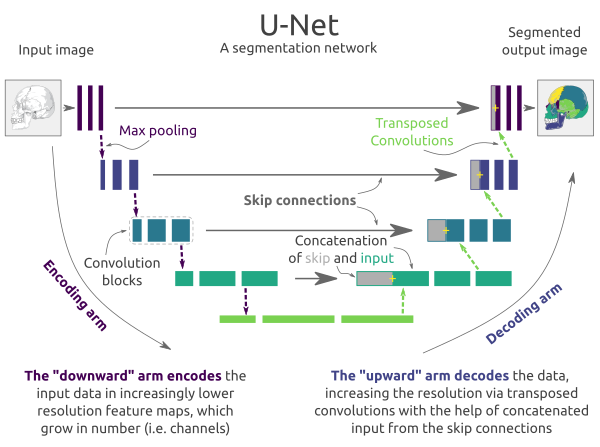
\includegraphics[width=1\linewidth]{img/unet_arquitectura.png}
    \caption{Estructura de la U-Net per a la separació d'àudio. Autor: \href{https://zefsguides.com/}{https://zefsguides.com/}}
    \label{fig:arquitectura-u-net}
\end{figure}

\paragraph{Aplicació de la U-Net en Separació d'Àudio}
L'arquitectura U-Net s'ha adaptat per a la separació de pistes d'àudio utilitzant espectrogrames com a entrada. Els espectrogrames proporcionen una representació visual del senyal d'àudio que la U-Net pot processar de manera efectiva.

\begin{itemize}
    \item \textbf{Entrada}: Espectrograma del senyal d'àudio mesclat.
    \item \textbf{Sortida}: Espectrogrames de les pistes d'àudio separades.
\end{itemize}

\paragraph{Exemple de Funcionament}
La U-Net s'entrena per aprendre a separar pistes específiques (com veus o instruments) del senyal d'àudio mesclat. Durant l'entrenament, la xarxa aprèn a identificar patrons de freqüència i temps que corresponen a cada pista.

\begin{itemize}
    \item \textbf{Exemple d'Entrenament}: Utilitzar una base de dades amb pistes d'àudio separades (per exemple, veus i música de fons) per entrenar la xarxa a identificar i separar aquestes pistes en nous àudios.
\end{itemize}

\paragraph{Avantatges i Desavantatges}
\begin{itemize}
    \item \textbf{Avantatges}:
        \begin{itemize}
            \item Pot capturar tant característiques locals com globals gràcies a la seva estructura en forma d'``U''.
            \item Utilitza connexions de pont per preservar informació de resolució alta durant tot el procés de decodificació.
        \end{itemize}
    \item \textbf{Desavantatges}:
        \begin{itemize}
            \item Requereix grans quantitats de dades d'entrenament anotades.
            \item Pot ser computacionalment costós en termes de memòria i temps de processament.
        \end{itemize}
    \end{itemize}

L'arquitectura U-Net és una eina potent per a la separació de pistes d'àudio gràcies a la seva capacitat per extreure i reconstruir característiques complexes. La seva aplicació en aquest camp ha demostrat ser efectiva, especialment quan s'utilitzen representacions visuals com els espectrogrames.


\subsection{Ús d'Espectrograms en la Separació d'Àudio}
Els espectrograms són una representació visual de l'espectre de freqüències d'un senyal d'àudio en funció del temps. Són fonamentals en molts dels mètodes de separació d'àudio moderns, ja que proporcionen una forma intuïtiva de visualitzar i analitzar les components freqüencials del senyal.

\paragraph{Definició i Càlcul dels Espectrogrames}
Un espectrograma es calcula aplicant la Transformada de Fourier de Curt Termini (STFT) al senyal d'àudio. Això implica dividir el senyal en finestres temporals superposades i aplicar la Transformada de Fourier a cada finestra per obtenir l'espectre de freqüències corresponent. Els resultats es combinen per formar una representació temps-freqüència.

\begin{itemize}
    \item \textbf{Formulació Matemàtica}: Si $x(t)$ és el senyal d'àudio, l'STFT $X(t, f)$ es defineix com:
    \[
    X(t, f) = \sum_{n=-\infty}^{\infty} x[n] \cdot w[n-t] \cdot e^{-j2\pi fn}
    \]
    on $w[n-t]$ és una finestra temporal centrada en $t$.
\end{itemize}

\paragraph{Magnitud i Fase}
La STFT genera valors complexos que poden ser descompostos en magnitud i fase. La magnitud indica la intensitat de cada freqüència en cada moment del temps, mentre que la fase indica la posició de la freqüència.

\begin{itemize}
    \item \textbf{Espectrograma de Magnitud}: Representa la intensitat de les freqüències, sovint visualitzada amb una escala de colors o en escala de grisos.
    \item \textbf{Espectrograma de Fase}: Més difícil de visualitzar, però essencial per a la reconstrucció precisa del senyal.
\end{itemize}

\paragraph{Aplicacions en Separació d'Àudio}
Els espectrograms són utilitzats per a crear màscares temps-freqüència que separen les components desitjades del senyal. Aquestes màscares poden ser binàries (on es manté una freqüència o es rebutja) o suaus (assignant un pes entre 0 i 1).

\begin{itemize}
    \item \textbf{Màscares Temps-Freqüència}: Utilitzades per filtrar components específics en un espectrograma. Per exemple, una màscara pot ser entrenada per eliminar soroll de fons deixant només la veu principal.
    \item \textbf{Predicció de la Fase}: Algoritmes com el de Griffin-Lim s'utilitzen per reconstruir la fase quan només es té la magnitud de l'espectrograma.
\end{itemize}

\paragraph{Espectrogrames en Deep Learning}
Els models de Deep Learning, com CNNs i U-Net, utilitzen espectrogrames com a entrada per aprendre a separar diferents fonts d'àudio. Aquests models poden extreure característiques complexes dels espectrogrames que són difícils de detectar amb mètodes tradicionals.

\begin{itemize}
    \item \textbf{Exemple d'Arquitectura U-Net}: Utilitza convolucions per identificar patrons en l'espectrograma, i convolucions transposades per reconstruir les pistes separades.
\end{itemize}

\begin{figure}[h]
    \centering
    \includegraphics[width=1\linewidth]{img/Especrtograma_harmònic.png}
    \caption{Exemple de la visualització d'un senyal d'àudio mitjançant l'espectrograma. Autor: Albertcastan, CC BY-SA 4.0.}
    \label{fig:espectrograma-harmonic}
\end{figure}

Els espectrogrames són una eina essencial en la separació de pistes d'àudio, proporcionant una representació visual rica en informació que és explotada per tècniques avançades de processament de senyal i Deep Learning. Les màscares temps-freqüència i les arquitectures de xarxes neuronals convolucionals són algunes de les tècniques que aprofiten les propietats dels espectrogrames per aconseguir una separació efectiva i precisa de les fonts d'àudio.


\subsection{Generació Automàtica de Partitures}
La generació automàtica de partitures és una altra àrea de recerca activa, amb aplicacions que van des de la transcripció musical fins a l'educació musical.

\paragraph{Symbolic Music Representation}
La representació simbòlica de la música, com MIDI, és utilitzada per generar partitures a partir d'àudio. Les tècniques modernes utilitzen models seqüència-a-seqüència per convertir espectrograms d'àudio en notació musical \cite{zeng2021musicbert}. Un exemple és el treball de Hawthorne et al. \cite{hawthorne2018enabling}, que utilitza un model seq2seq per a la transcripció automàtica de piano.

\begin{itemize}
    \item \textbf{Avantatges}: Pot generar partitures detallades i editables.
    \item \textbf{Desavantatges}: Pot ser limitat per la precisió del model i la complexitat del senyal d'entrada.
\end{itemize}

\paragraph{Transcription Models}
Els models de transcripció automàtica de música utilitzen xarxes neuronals per identificar les notes i altres esdeveniments musicals en un enregistrament d'àudio. Això inclou tant els mètodes basats en CNN com els basats en RNN, així com les arquitectures híbrides que combinen les dues \cite{sturm2016music}. El model Onsets and Frames \cite{hawthorne2017onsets} és un exemple destacat que utilitza CNNs per detectar els inicis de les notes i RNNs per identificar la durada de les notes.

\begin{itemize}
    \item \textbf{Avantatges}: Alta precisió en la detecció de notes i esdeveniments musicals.
    \item \textbf{Desavantatges}: Requereix grans quantitats de dades d'entrenament i pot ser afectat pel soroll de fons.
\end{itemize}

En resum, la combinació de mètodes clàssics i moderns, juntament amb els avenços en Deep Learning, han permès progressos significatius en la separació de pistes d'àudio i la generació automàtica de partitures. Aquest treball busca aprofitar aquestes tècniques per proporcionar una plataforma avançada per a l'anàlisi i generació de partitures musicals.


\section{Desenvolupament}

El desenvolupament del projecte s'ha separat en 4 grans apartats. Inicialment, la generació i neteja de dades, a continuació, la separació d'àudio en pistes, continuant amb l'anàlisi de la pista obtenint les notes en format MIDI per a finalment generar la partitura donat aquest arxiu.

\subsection{Dades}

Les dades es separen en diversos grups segons la seva finalitat d'ús.

\subsubsection{Elements Simples i Problemes Simples}

Els elements simples consisteixen en sons senzills d'un mateix instrument tocant una sola nota o una melodia simple. La duració màxima d'aquestes dades és de 5 segons.

Per tal de tenir una visió més àmplia, he creat els elements simples personalment. Els he realitzat mitjançant programes de software lliures que permeten produir música amb l'ordinador. He triat diversos instruments amb les seves variacions per tal de crear múltiples elements simples.
El problema o inconvenient d'aquesta manera de treballar és el cost temporal. Crear els elements simples manualment requereix molt temps, per això és necessària alguna manera d'augmentar el nombre de dades d'una manera més senzilla.

Amb l'objectiu de solucionar aquesta problemàtica, elements simples s'introdueixen en un bloc de codi que anomenem ``generador''. Aquest generador agrupa un o més elements simples per crear els \textbf{problemes simples}. Els problemes simples són el resultat d'agrupar els elements simples i modificar-los mitjançant els valors de diverses variables del generador. Les variables d'ajust són: \(\alpha\), \(\beta\), volum1 i volum2, amb les quals es crea i modifica un àudio estèreo per variar el volum dels canals dret i esquerre, així com desplaçar en l'eix temporal el senyal d'àudio i afegir soroll. Aquests valors permeten generar moltes dades diferents amb pocs recursos (elements simples). 
Aquesta metodologia permet que amb pocs elements simples, tingui la capacitat de crear molts problemes simples (+500) diferents.

Per mantenir la base de dades senzilla i de mida petita, els problemes simples no s'enregistren; simplement s'enregistra la seva llavor (seed) de creació, que consta dels valors de les variables i dels elements simples utilitzats. Això minimitza l'espai en disc, ja que els problemes simples es poden recrear a demanda.

L'esquema de creació dels problemes simples és el següent: \ref{fig:data-generator-formula}
\begin{figure}[h]
    \centering
    
\includegraphics[width=1\linewidth]{img/data_generator_formula.png}
    \caption{Esquema de creació de problemes simples}
    \label{fig:data-generator-formula}
\end{figure}

\subsubsection{Elements Complexos i Problemes Complexos}

Els elements complexos, de manera similar als problemes simples, s'utilitzen per generar els \textbf{problemes complexes}. Aquests problemes estan formats per melodies més complexes amb l'objectiu de tenir àudios d'entrenament més fidels a la realitat, com ara cançons del mercat o similars.

Els elements complexes s'han creat de la mateixa manera que els simples, mitjançant un programa de producció musical. Els àudios conten notes i melodia més complexes de cada instrument.

\subsubsection{Àudios Reals}

Els àudios reals consisteixen en enregistraments d'àudios com concerts, gravacions de mòbil, etc. Aquest tipus de dades només s'utilitzen per a la part de test, ja que el model no s'entrena amb aquestes dades.

En resum, el projecte utilitza diversos tipus de dades segons la finalitat. Hi ha dades (elements simples i complexes) que s'utilitzen per generar la base de dades utilitzada en els algoritmes (problemes simples i complexes). Addicionalment existeixen els àudios reals, els quals només es poden utilitzar de test. 

Les dades utilitzades són fruit de les dades creades per mi o generades pel meu codi. Tot i això, per millorar la qualitat de les dades i basar-me en un dataset públic, famós i utilitzat mundialment, utilitzaré per alguns resultats addicionals la base de dades \textbf{musdb18} \cite{musdb18}, que conté més de deu hores de música dividida en diverses pistes.



\subsection{Separació d'àudio}

Per a la separació d'àudio, he aplicat dos mètodes diferents dels prèviament explicats a ``l'Estat de l'Art'' amb l'objectiu d'analitzar i comparar els resultats obtinguts.

El primer mètode utilitzat és un algoritme clàssic, basat en l'algoritme de Independent Component Analysis (ICA). L'ICA és un mètode amplament utilitzat per a la descomposició de l'àudio en les seves fonts originals. Aquest algoritme té com a objectiu la separació de les senyals d'entrada en diferents components independents. En aquest cas, s'utilitzarà l'ICA per aconseguir la separació d'un àudio en pistes individuals.

D'altra banda, per als algoritmes actuals, s'utilitza un mètode basat en tècniques de Deep Learning (DL). S'utilitza l'arquitectura U-Net \cite{spleeter2020}. La U-Net és àmpliament utilitzada en tasques de processament d'àudio i imatge per a la segmentació i reconstrucció d'imatges.

Per a poder analitzar el rendiment d'aquests mètodes amb les màximes variacions possibles, es poden utilitzar diverses formes de processament d'àudio. Per tal de facilitar l'aplicació d'aquestes, la metodologia que es segueix és la programació de blocs o ``caixes'' intercanviables. D'aquesta manera, s'aconsegueix un codi més flexible i reutilitzable.

Aquesta manera de treballar permet utilitzar una o més formes de processament de manera senzilla, la qual cosa és útil per a poder comparar resultats o estudiar i analitzar en quins casos rendeix millor un algoritme amb una forma de processament concreta.

Aquestes formes de processament són \cite{audio-processing-ML}:

\begin{itemize}
\item \textbf{Spectrum:} Anàlisi de l'espectre de freqüències de l'àudio.
\item \textbf{Cepstrum:} El cepstrum d'un senyal és el resultat de calcular la Transformada de Fourier de l'espectre del senyal estudiat mesurat en escala logarítmica (dB), i és utilitzat per a la representació de la informació d'una manera més robusta enfront de la reverberació i el soroll.
\item \textbf{MFCC (Mel Frequency Cepstral Coefficients):} Coeficients cepstrals de les freqüències mel, amplament utilitzats en el reconeixement de veu i altres tasques de processament d'àudio.
\item \textbf{GFCC (Gammatone Frequency Cepstral Coefficients):} Coeficients cepstrals de les freqüències gammatone, una representació més semblant al processament auditiu humà.
\end{itemize}

Aquestes formes de processament permeten un anàlisi detallat dels resultats obtinguts mitjançant diferents mètodes i tècniques, ajudant a determinar quin és l'enfocament més adequat per al problema de separació d'àudio en el marc d'aquest projecte.

\subsection{Algoritme clàssic - Independent Component Analysis (ICA)}

Per a entendre millor l'algoritme, ja que inicialment l'absència de coneixement m'acompanyava durant el dia a dia, vaig començar a implementar-lo seguint les fórmules matemàtiques.
Un cop familiaritzat amb l'algoritme, ja he estat capaç d'utilitzar FastICA \cite{langlois2010introduction} de sklearn, el qual aporta funcions ja optimitzades que implementen aquest algoritme clàssic de manera ràpida. 

\subsubsection{Preprocessament Inicial}

Degut a que l'algoritme ICA és un algoritme clàssic i no està basat en un model de Deep Learning, sinó en operacions matemàtiques, no cal entrenar prèviament el model; la qual cosa implica que les dades a estudiar es poden introduir directament.

Tot i això, l'àudio en format .wav prèviament s'ha de processar en format d'espectrograma


\subsubsection{Aplicació de l'Algoritme ICA}

L'aplicació de l'algoritme ICA segueix aquests passos:

\begin{itemize}
    \item \textbf{Centrat i blanqueig:} Les dades d'entrada es centren (es resten les mitjanes) i es blanquegen (transformació per obtenir components no correlacionades amb variància unitària).
    \item \textbf{Estimació de components independents:} Utilitzant un algoritme iteratiu, com FastICA, es maximitza la no-Gaussianitat de les dades transformades per obtenir els components independents $\mathbf{S}$.
    \item \textbf{Reordenació i escalat:} Els components recuperats es poden reordenar i escalar per correspondre millor amb les fonts originals.
\end{itemize}

\subsubsection{Avaluació del Rendiment}

L'avaluació del rendiment de l'algoritme ICA es pot dur a terme mitjançant diverses mètriques, com ara la correlació entre les components separades i les fonts originals, el coeficient de determinació (R²), i altres mesures de qualitat de senyal.

\subsubsection{Anàlisi de Resultats i Limitacions}

Després de l'aplicació de l'algoritme ICA, els resultats obtinguts es comparen amb les fonts originals per avaluar l'eficàcia de la separació. L'anàlisi de resultats inclou la identificació de limitacions de l'algoritme, com ara la seva sensibilitat al soroll i la dificultat per separar fonts que no siguin suficientment independents.

Aquest enfocament permet una comprensió detallada de com l'algoritme ICA pot ser aplicat en la descomposició d'àudio i proporciona una base sòlida per comparar-ne el rendiment amb altres mètodes, com les xarxes neuronals convolucionals amb arquitectura U-Net que es veurà més endavant.

\subsection{Algoritme actual - Deep Learning (CNN, U-Net)}

El procés de desenvolupament de l'algoritme de descomposició d'àudio es basa en l'ús d'una xarxa neuronal convolucional (CNN) amb una arquitectura U-Net. L'objectiu principal és entrenar el model per separar les diferents components d'un senyal d'àudio complex, format per la combinació de sons simples.

\subsubsection{Preprocessament Inicial}

Inicialment comptem amb unes dades simples (SimpleElements), que consisteixen en sons individuals d'instruments, utilitzant el generador es creen problemes simples, que serviran com a dades d'entrenament. Aquest generador s'ha modificat respecte al plantejat anteriorment per a realitzar els canvis aleatoris realitzats als problemes simples també als elements simples. D'aquesta manera s'obtenen els valors de \textit{ground truth}. Posteriorment, es divideixen els problemes simples en tres subconjunts: entrenament, validació i test.

\subsubsection{Entrenament del Model}

L'entrenament del model implica la configuració de diversos paràmetres com el nombre de \textit{batches} d'entrenament \textit{(train\_batches)}, la mida del batch \textit{(batch\_size)} i el nombre total d'èpoques \textit{(epochs)}. Durant cada època, es segueix el següent procediment:

\begin{itemize}
    \item Per a cada \textit{batch} d'entrenament, es generen àudios complexos i els seus corresponents resultats \textit{(ground truth)} mitjançant el generador.
    \item Aquests àudios es converteixen en espectrogrames.
    \item Els espectrogrames s'ajusten a la mida adequada i es processen en forma de \textit{batch} per entrenar el model.
\end{itemize}

Després de processar els batches d'entrenament, es procedeix de manera similar amb els batches de validació per avaluar el rendiment del model durant l'entrenament.

\subsubsection{Avaluació Final}

Un cop completades totes les èpoques d'entrenament, s'utilitza el conjunt de test per avaluar el rendiment del model de manera objectiva. Les mètriques d'avaluació calculades inclouen l'exactitud, la precisió, el recall i el F1-score, entre d'altres.

\subsubsection{Anàlisi de Resultats i Ajustament del Model}

Finalment, els resultats obtinguts es revisen per identificar els punts forts i febles del model. Aquest anàlisi permet ajustar els hiperparàmetres i refinar l'arquitectura del model per millorar-ne el rendiment.

Aquest procés iteratiu assegura que el model s'entreni de manera òptima, es validi per evitar el sobreajustament i es testi per garantir una avaluació precisa del seu rendiment global.


\subsection{Transcripció d'àudio}

Donada una de les pistes obtingudes en la separació d'àudio, és a dir un sol instrument, es realitza una transcripció de les notes en format MIDI. D'aquesta manera, es coneix la durada de cada nota i la seva posició temporal. \cite{music-transcription-app132111882} 

Per al desenvolupament d'aquesta part m'he basat en Omnizard \cite{Omnizard-Wu2021}, doncs ha estat amb el que he obtingut millors resultats.


\subsection{Generació de partitura}

Per a la generació de partitures, he estat fent recerca i provant les llibreries music21 \cite{music21-conf/ismir/CuthbertA10} i partitura \cite{partitura_mec}.

En aquest context, s'ha obtingut millors resultats amb la llibreria music21, però s'explorarà amb més profunditat la llibreria partitura.

L'objectiu d'aquesta subsecció és generar la partitura de cada pista o instrument obtingut mitjançant el procés de separació d'àudio.

\section{Resultats}
Per tal d'expressar de la millor manera possible els resultats, es separen en diverses subseccions per tal d'aprofundir més en detall segons la seva finalitat. Primerament es fa l'anàlisi dels resultats referents a la descomposició d'àudio, on els algoritmes ICA i l'arquitectura U-Net són els protagonistes.
A continuació 

\subsection{Audio Decomposition}

En aquesta secció es descriuen les mètriques utilitzades per avaluar els resultats dels algoritmes clàssic ICA i Deep Learning amb arquitectura U-Net, així com les expectatives de rendiment de cadascun.

\subsection{Mètriques Quantitatives}

Per avaluar la qualitat de la descomposició d'àudio, es poden utilitzar les següents mètriques quantitatives:

\begin{itemize}
    \item \textbf{Relació Senyal-Soroll (SNR):} \cite{Johnson:2006_SNR} Aquesta mètrica mesura la qualitat de la separació de les fonts. Un SNR més alt indica una millor qualitat de separació.
    
    \item \textbf{Correlació Creuada:} Mesura la similitud entre les fonts separades i les fonts originals. 
    
    \item \textbf{Coeficient de Determinació (R²):} \cite{akossou2013impact_r_squared} Aquesta mètrica mesura la proporció de la variància de les fonts originals explicada per les fonts separades.
    
    \item \textbf{Mean Squared Error (MSE):} \cite{5937917_MSE} Mesura la diferència quadrada mitjana entre les fonts separades i les fonts originals.
\end{itemize}

\subsection{Anàlisi Qualitatiu}

A més de les mètriques quantitatives, es pot realitzar un anàlisi qualitatiu per avaluar altres aspectes de la qualitat de la separació de les fonts:

\paragraph{Qualitat Subjectiva de l'Àudio:} Es farà una avaluació de la qualitat perceptiva de les fonts separades mitjançant proves d'escolta humana. 

% Petita conclusió
En resum, tot i que l'algoritme ICA és una tècnica clàssica robusta per a la separació de fonts, la CNN amb U-net s'espera que superi l'ICA en diverses mètriques clau gràcies a la seva capacitat per aprendre característiques complexes i no lineals de les dades d'àudio. S'espera que l'arquitectura U-net ofereixi una millor qualitat de separació, robustesa al soroll i capacitat de generalització, fent-la una opció més adequada per a tasques de descomposició d'àudio en entorns complexos.

\subsection{Exemple d'execució de l'ICA}

He realitzat un exemple d'execució de l'algoritme ICA amb resultats audibles en un Google Colab. A continuació adjunto dos links, el primer és el del codi i el segon és el de les dades necessàries per tal de fer l'execució i els resultats de la mateixa.

Per veure un codi d'exemple ICA amb 3 àudios, visita aquest enllaç:
\url{https://colab.research.google.com/drive/14PoGcjAzsykyX0y72bGA1_LEaXnj3HTC?usp=sharing}

Les dades d'input i output es poden trobar en aquest enllaç:
\url{https://github.com/PolKinsa/TFG_PolColomerCampoy/tree/main/Exemples/ICA_3_example_audios}

En aquest exemple es poden escoltar 3 àudios d'entrada corresponents a una gravació d'un mateix concert però cada gravació està feta des d'un punt diferent. En alguna d'elles inclús hi ha soroll afegit.

Una vegada s'executa l'algoritme, podem observar escoltant els àudios que en el resultat 2 s'ha separat correctament el piano i en el resultat 3 s'ha separat correctament el violoncel, tot i que de fons cap a la meitat de l'àudio s'escolta una mica de soroll.
En el resultat 1 s'ha separat el soroll que s'havia afegit, tot i que també s'escolta, en volum molt baix, el piano. Per tant, no s'ha realitzat la separació amb una qualitat excepcional.

A continuació mostro els espectrogrames resultants de l'execució.
\ref{fig:ica-exemple-3-audios}
\begin{figure}[h]
    \centering
    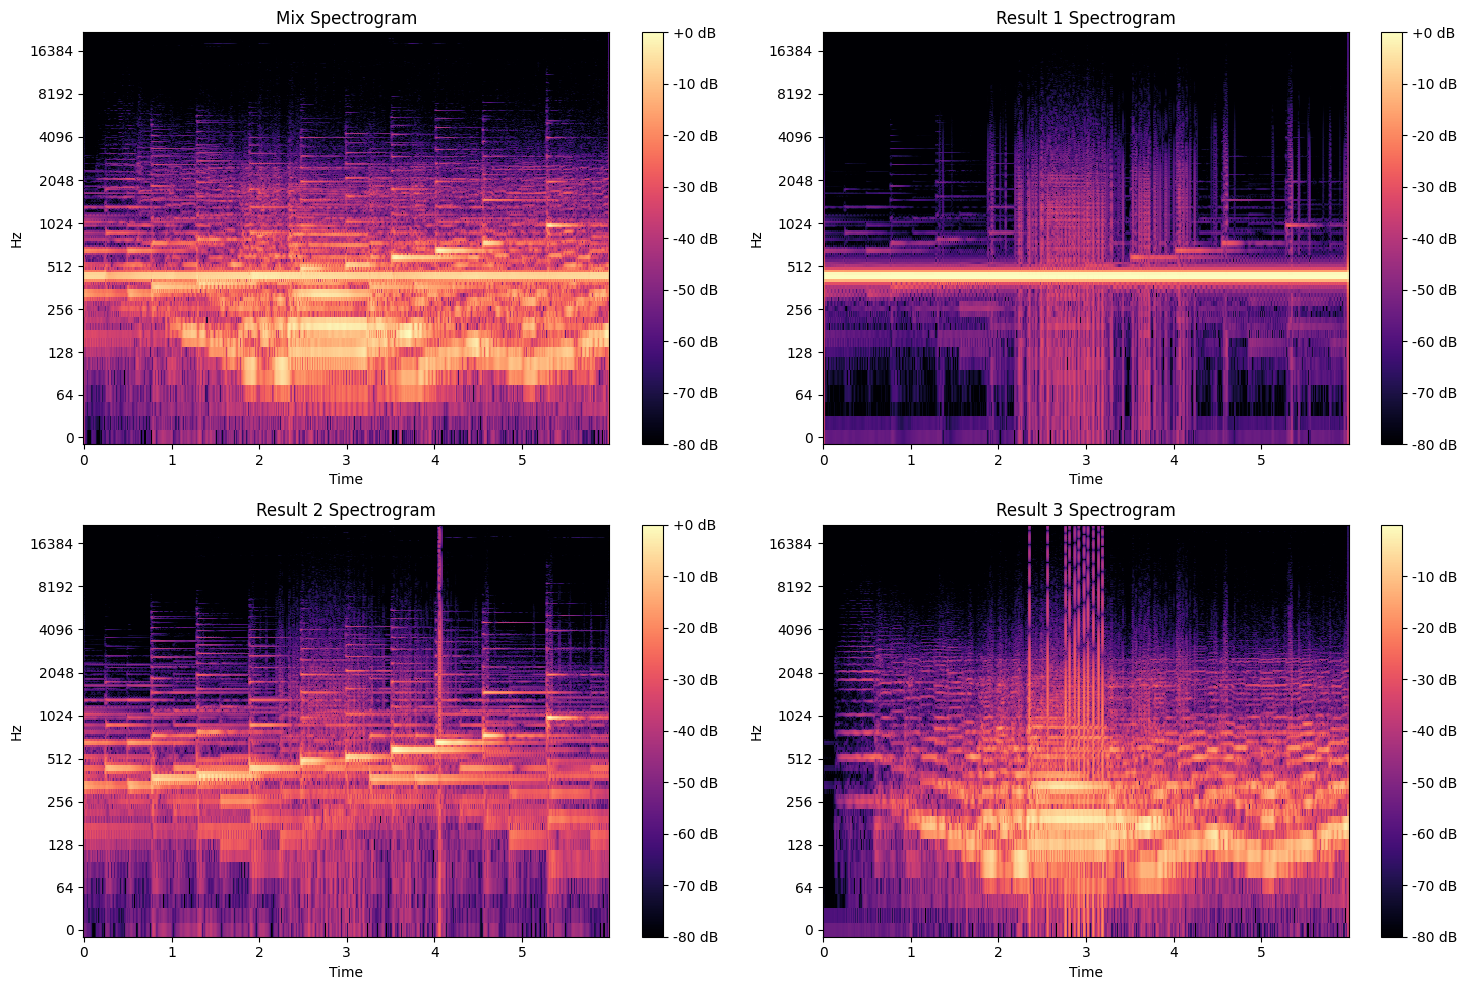
\includegraphics[width=1\linewidth]{img/ica_results/resultICA.png}
    \caption{Resultat dels espectrogrames de l'exemple de 3 àudios de l'execució de l'algoritme ICA.}
    \label{fig:ica-exemple-3-audios}
\end{figure}
Primerament podem observar el espectrograma ``Mix 1'', referent a un dels inputs i a continuació els tres resultats, referent a les 3 pistes en les que s'ha separat el ``Mix 1''.

\subsection{Exemple d'execució d'U-Net}

Seguint la mateixa estructura que l'exemple anterior, mostro a continuació un exemple de la U-Net utilitzant ``spleeter'' \cite{spleeter2020}.

Per veure un codi d'exemple de l'arquitectura U-Net, visita aquest enllaç:
\url{https://colab.research.google.com/drive/1MzaPNfZnVwvhG4f_C-HInDPgy7sN7j4J?usp=sharing}

Les dades d'input i output es poden trobar en aquest enllaç:
\url{https://github.com/PolKinsa/TFG_PolColomerCampoy/tree/main/Exemples/UNET_example}

D'igual manera que amb la U-Net, a continuació mostro l'espectrograma resultant de la descomposició de l'àudio, doncs aquest és una imatge i es pot plasmar en el paper/pantalla, no com l'àudio. Tot i això, recomano encaridament escoltar els àudios resultants de l'execució en el Google Colab. 

\ref{fig:U-Net-exemple}
\begin{figure}[h]
    \centering
    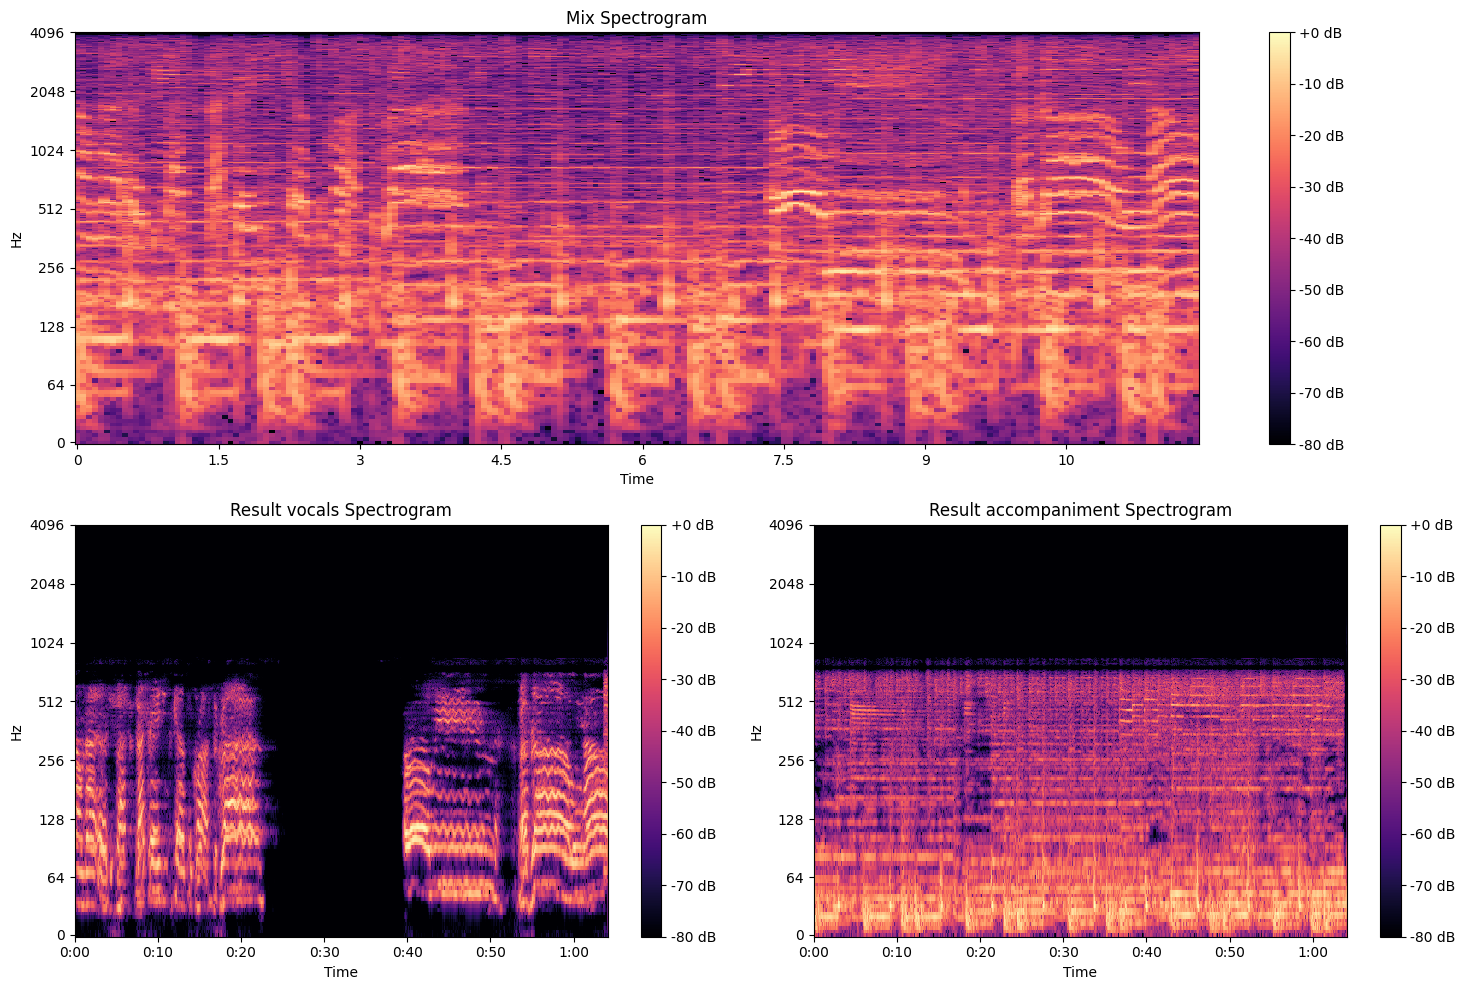
\includegraphics[width=1\linewidth]{img/u-net_results/unet_example.png}
    \caption{Resultat dels espectrogrames de l'exemple de l'arquitectura U-Net.}
    \label{fig:U-Net-exemple}
\end{figure}

La qualitat d'aquesta separació en pistes és molt bona, sobretot la pista resultant d'acompanyament, doncs la pista de la veu tot i estar molt ben separada sí que sembla que s'escolta amb una mica d'eco.
Tot i això la qualitat és molt bona per no dir excepcional, i té un millor rendiment que l'algoritme ICA.

\subsection{Transcripció musical i generació de partitura}

En el cas de la transcripció musical i generació de partitura he fet el següent. Primerament mitjançant un programa de producció musical he creat una melodia simple de piano de ``DO, RE, MI, RE'' de notes negres.

A continuació he exportat el .mp3 i també el .mid, d'aquesta manera tinc l'arxiu d'àudio i la seva corresponent transcripció.
Mitjançant Omnizard \cite{Omnizard-Wu2021}, es pot realitzar la transcripció d'un arxiu .mp3 o video de YouTube a .mid (MIDI). 
A continuació adjunto el link al codi d'exemple de generació de partitura:
\url{https://colab.research.google.com/drive/1tiGLzMGYfOxaYQx5lRwElC0yLjdWvwAU?usp=sharing}
Dades utilitzades (.mp3 i .mid):
\url{https://github.com/PolKinsa/TFG_PolColomerCampoy/tree/main/Exemples/ExempleGeneraci%C3%B3Partitura}

\ref{fig:generacio-partitura-exemple-doremire}
\begin{figure}[h]
    \centering
    
\includegraphics[width=1\linewidth]{img/generacioPartituraDoReMiRe.png}
    \caption{Resultat de la generació de la partitura (``DO, RE, MI, RE''.}
    \label{fig:generacio-partitura-exemple-doremire}
\end{figure}

Tal i com es pot veure en aquesta petita partitura, el resultat és correcte.

Addicionalment, he realitzat una prova molt més exhaustiva amb la cançó d'aquest enllaç de YouTube: \url{https://www.youtube.com/watch?v=aCUI6dNECeA&ab_channel=tocapartituras.com}
\begin{figure}[h]
    \centering
    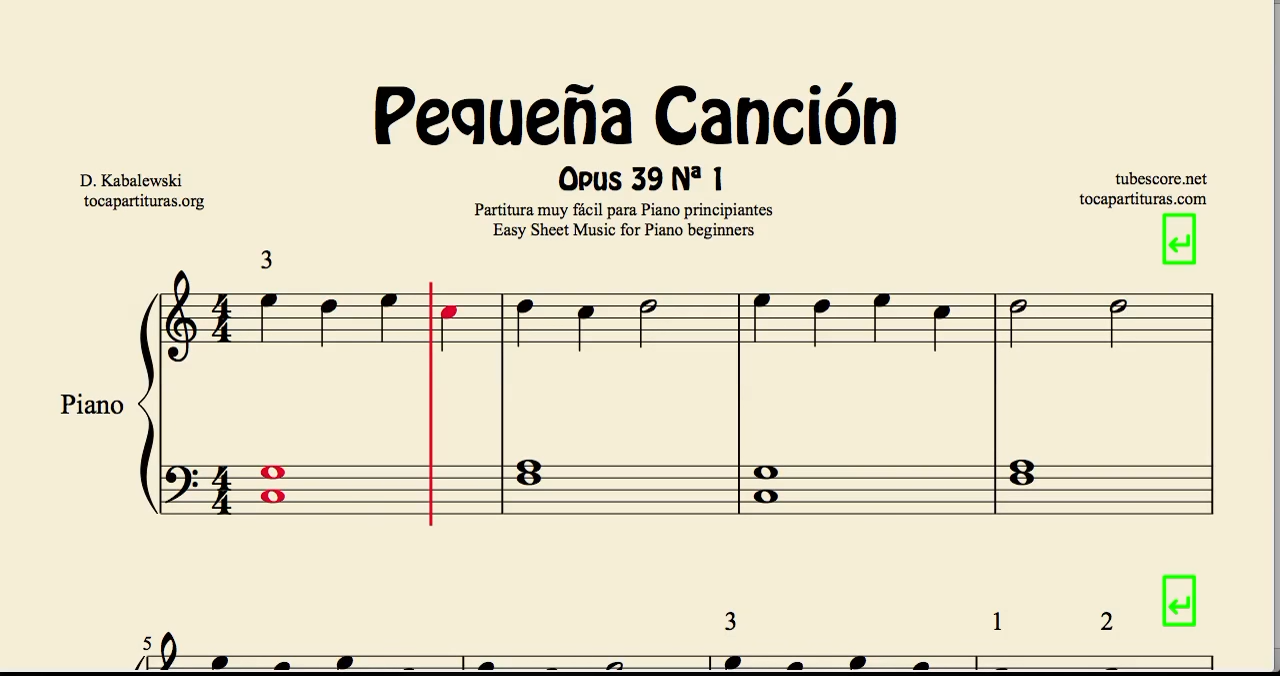
\includegraphics[width=1\linewidth]{img/screenshot-partitura-correcta.png}
    \caption{Partitura original del video de YouTube.}
    \label{fig:paritura-original}
\end{figure}
Com es pot observar, aquesta cançó és més complexa que l'exemple anterior donat, i conté partitura per a la mà dreta i per a la mà esquerra alhora. \ref{fig:paritura-original}


I a continuació podem veure la partitura generada: \ref{fig:partitura-resultat}
\begin{figure}[h]
    \centering
    
\includegraphics[width=1\linewidth]{img/partitura_resultat.png}
    \caption{Partitura resultant, generada al Google Colab 2.}
    \label{fig:partitura-resultat}
\end{figure}

Com es pot observar, el resultat és desastrós i molt diferent. 
El procés de transcripció de video de YouTube cap a arxiu .mid amb Omnizard i la generació de la partitura amb la llibreria music21 \cite{music21-conf/ismir/CuthbertA10}, no s'ha realitzat correctament.
Tot i això es veu que és possible una generació de partitura, se li haurà de dedicar més temps a entendre com funciona si en un futur es vol realitzar la generació de partitures amb les dues mans, en el cas del piano. Tal i com es pot veure, la partitura original era amb les dues mans, però el resultat només ha considerat la mà dreta (melodia), la qual cosa pot ser el punt principal d'error fent que es desquadri tant.

\section{Conclusions}

L'algorisme ICA és un mètode clàssic que va ser pioner i efectiu en la seva època inicial d'implementació. Tot i que proporciona una certa distinció i separació de les pistes, la seva qualitat no és excel·lent. Per aquell temps, era suficient per discernir les diferències, tot i que el soroll podia ser evident; un arxiu resultant encara podia identificar principalment un únic instrument en l'àudio.

No obstant això, com s'ha esmentat, la seva qualitat general és limitada. Això ha portat al desenvolupament i la adopció de noves tecnologies, com els models basats en aprenentatge automàtic, que ofereixen una millor qualitat i precisió.

En aquest projecte, s'ha optat per utilitzar un model actual basat en l'arquitectura U-Net, el qual ha demostrat ser eficaç per a la segmentació d'imatges. Encara que aquest model està dissenyat per a imatges, s'ha aplicat a àudio transformant-lo prèviament en format d'espectrograma.

Aquesta decisió ha comportat diversos reptes i complicacions. La transformació d'àudio a un format d'imatge adient per a la entrada del model U-Net no és trivial, especialment per a algú sense experiència prèvia.

Així doncs, és essencial considerar els reptes potencials abans d'emprendre un projecte d'aquest tipus. Per a un principiant com jo, la implementació d'aquest model ha representat un desafiament considerable.

Per tant, és important reconèixer que l'algorisme ICA, malgrat les seves limitacions, és més senzill d'implementar, tot i que els resultats poden ser inferiors. En contrapartida, models més avançats com l'arquitectura U-Net prometen resultats superiors, però la seva implementació pot ser notablement més complexa.

No sempre uns resultats superiors es tradueixen en una major complexitat d'implementació; sovint reflecteixen tècniques més eficaces i millor desenvolupades. Tanmateix, en el meu cas personal, la implementació d'aquest model ha implicat una dificultat addicional significativa.

\subsection{Future work}

Tal i com he comentat en la introducció, aquest TFG forma part de l'inici d'un projecte més gran, que pretén apropar la música a tothom.
Per tal de continuar aquest projecte, s'hauria de seguir estudiant la descomposició d'àudio i generació de partitures per tal de fer-les més eficients i òptimes. Addicionalment, m'encantaria trobar alguna manera per poder crear tutorials visuals per a cada instrument, per tal de facilitar el procés d'aprenentatge.

\section*{Agraïments}

Vull agrair a molta gent pel fet d'estar al meu costat durant tots aquests mesos.
Aquest projecte ha sigut llarg i frustant a estones, doncs no comptava amb el coneixement inicial per portar-lo a terme. Vull agrair a la meva familia, parella i amics per animar-me i fer-me companyia, ajudant-me a desconnectar.

Al meu tutor del TFG per a les reunions i facilitar-me horaris per poder fer un seguiment.

I finalment a Internet per tota la informació disponible que m'ha permès fer la recerca necessària per dur a terme aquest treball.


\bibliographystyle{plain}
\bibliography{biblio}



\end{document}

